\documentclass[11pt,a4paper]{article}

% =========================================================
% PACKAGES
% =========================================================

\usepackage[margin=0.8in]{geometry}
\usepackage{booktabs}
\usepackage{array}
\usepackage{enumitem}
\usepackage{hyperref}
\usepackage{float}
\usepackage{tikz}
\usepackage{titlesec}
\usepackage{setspace}

\usetikzlibrary{positioning,arrows.meta}

% =========================================================
% DOCUMENT FORMATTING
% =========================================================

\hypersetup{
    colorlinks=true,
    linkcolor=black,
    urlcolor=blue
}

\setlength{\parindent}{0pt}
\setlength{\parskip}{5pt}

\onehalfspacing

\titleformat{\section}
{\large\bfseries}
{\thesection.}
{0.5em}
{}

\titleformat{\subsection}
{\normalsize\bfseries}
{\thesubsection.}
{0.5em}
{}

\setlist[itemize]{
    noitemsep,
    topsep=2pt,
    leftmargin=1.5em
}

\setlist[enumerate]{
    noitemsep,
    topsep=2pt,
    leftmargin=1.7em
}

% =========================================================
% DOCUMENT
% =========================================================

\begin{document}

% =========================================================
% TITLE
% =========================================================

\begin{center}

{\Large \textbf{THAPAR TRADE}}\\[0.25cm]

{\large
\textbf{A Campus Marketplace for Student-to-Student Trading}
}\\[0.45cm]

{\normalsize
Rajbir Singh -- 1024030453\\
Chitesh Jindal -- 1024030454\\
Ishan Garg -- 1024031095
}\\[0.3cm]

{\normalsize
Thapar Institute of Engineering and Technology
}\\[0.15cm]

{\normalsize
UCS503P -- Project Proposal
}\\[0.15cm]

{\normalsize
August 2026
}

\end{center}

\vspace{0.15cm}
\hrule
\vspace{0.2cm}

% =========================================================
% 1. INTRODUCTION / PROBLEM STATEMENT
% =========================================================

\section{Introduction and Problem Statement}

Student-to-student exchange of used products is a common
requirement within a university environment. At Thapar, students
may need to buy or sell textbooks, calculators, cycles,
electronics, furniture, hostel appliances and other academic or
personal items. These transactions are currently facilitated
largely through informal channels such as WhatsApp groups, ION
groups, personal contacts and word of mouth.

Although these channels enable communication, they do not provide
the functionality of a structured marketplace. Product
information becomes distributed across multiple conversations,
making relevant listings difficult to discover. Buyers cannot
reliably search or filter products by category, price, condition
or availability. Sellers may also fail to update or remove
listings after an item has been sold, resulting in unnecessary
communication and inaccurate availability information.

A further challenge is the reliability of marketplace listings.
For example, a student may jokingly or misleadingly list a
product belonging to another student as if it were their own,
even though the actual product is not for sale. A general
marketplace does not provide a campus-specific mechanism through
which such listings can be reported and reviewed.

\textbf{Thapar Trade} proposes a centralized, campus-specific
marketplace that addresses these limitations through structured
product listings, student authentication, search and filtering,
availability management, reporting and administrative moderation.
Students will be able to report listings that they believe are
unauthorized, misleading or falsely claim ownership. Reported
listings can then be reviewed by an administrator and removed or
restored as appropriate.

The project therefore aims to make student-to-student trading
more organized, searchable and reliable while providing a
practical mechanism for handling misleading or unauthorized
listings.

% =========================================================
% 2. OBJECTIVES
% =========================================================

\section{Objectives}

The primary objective is to design and implement a functional
campus marketplace that provides a structured workflow for
student-to-student trading.

The project will pursue the following objectives:

\begin{itemize}

    \item Develop an authenticated web platform through which
    students can create, browse and manage product listings.

    \item Implement keyword-based search and filtering by
    category, price, condition and availability.

    \item Implement listing states of \textit{Available},
    \textit{Reserved} and \textit{Sold} to maintain accurate
    product availability.

    \item Provide structured product information including
    descriptions, prices, conditions and images.

    \item Implement a reporting mechanism for suspicious,
    misleading or unauthorized listings.

    \item Develop an administrative moderation interface for
    reviewing reports and taking appropriate action.

    \item Validate the system through functional testing and
    user-acceptance testing with a small group of student users.

\end{itemize}

The project will prioritize a complete and reliable core
marketplace before considering advanced functionality.

% =========================================================
% 3. METHODOLOGY
% =========================================================

\section{Methodology}

The project will follow an iterative software-engineering
methodology in which the system is developed as a set of
integrated functional modules. The methodology will cover
architecture design, module implementation, system integration,
testing and validation.

\subsection{System Architecture}

The proposed system will use a three-layer architecture
consisting of a presentation layer, application layer and data
layer.

\begin{center}

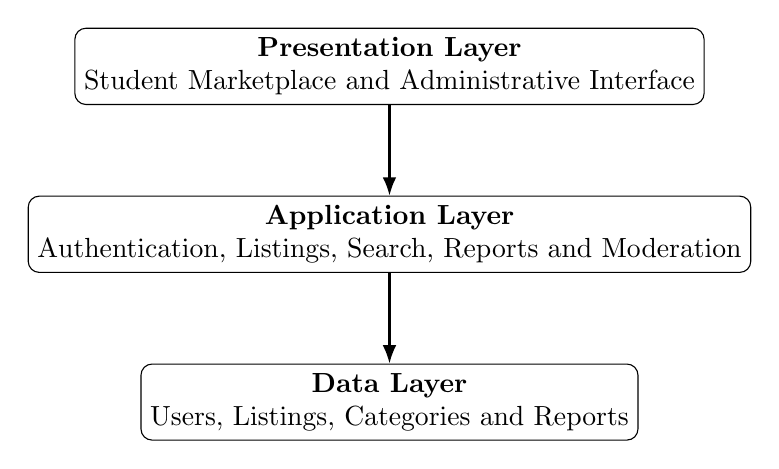
\begin{tikzpicture}[
    node distance=1.15cm,
    box/.style={
        draw,
        rounded corners,
        minimum width=5.4cm,
        minimum height=0.8cm,
        align=center
    },
    arrow/.style={
        -{Latex},
        thick
    }
]

\node[box] (frontend)
{\textbf{Presentation Layer}\\
Student Marketplace and Administrative Interface};

\node[box, below=of frontend] (backend)
{\textbf{Application Layer}\\
Authentication, Listings, Search, Reports and Moderation};

\node[box, below=of backend] (database)
{\textbf{Data Layer}\\
Users, Listings, Categories and Reports};

\draw[arrow] (frontend) -- (backend);
\draw[arrow] (backend) -- (database);

\end{tikzpicture}

\end{center}

The presentation layer will provide responsive interfaces for
students and administrators. The application layer will
implement authentication, listing management, search, reporting
and moderation logic. The data layer will maintain structured
records for users, listings, categories and reports.

The final implementation technologies will be selected according
to team familiarity, development requirements and availability of
appropriate free or academic-tier services.

\subsection{Functional Modules}

The system will be implemented through the following modules:

\begin{itemize}

    \item \textbf{Authentication and User Management:}
    The platform will associate marketplace activity with an
    authenticated student account.

    \item \textbf{Product Listing:}
    Sellers will provide standardized information including
    product title, category, description, price, condition and
    images. Required fields will be validated before publication.

    \item \textbf{Marketplace Search:}
    Students will be able to search listings using keywords and
    refine results using category, price, condition and
    availability filters.

    \item \textbf{Listing Lifecycle:}
    Sellers will manage product availability using
    \textit{Available}, \textit{Reserved} and \textit{Sold}
    states.

    \item \textbf{Product Details and Seller Information:}
    Buyers will be able to view product information, listing
    condition, price and relevant seller information before
    contacting the seller.

    \item \textbf{Reporting Mechanism:}
    Users will be able to report listings that they believe are
    misleading, unauthorized, inappropriate or falsely claim
    ownership.

    \item \textbf{Administrative Moderation:}
    Administrators will review submitted reports and may
    temporarily restrict, remove or restore listings based on
    the review.

\end{itemize}

\subsection{Reporting and Moderation Workflow}

The reporting mechanism is designed to address cases in which a
student lists another student's product without authorization,
including misleading or prank listings.

A user can select ``Report Listing'' from the product page and
choose a relevant reason, such as:

\begin{itemize}

    \item Product is not for sale.
    \item I am the actual owner.
    \item Seller is falsely claiming ownership.
    \item Product information is misleading.
    \item Other.

\end{itemize}

The report will be stored in the database and made available to
the administrator through the moderation dashboard.

The workflow will be:

\begin{center}

\textbf{Listing}
$\rightarrow$
\textbf{Report}
$\rightarrow$
\textbf{Administrative Review}
$\rightarrow$
\textbf{Restore or Remove}

\end{center}

This approach does not require every student to register their
personal possessions in advance. Instead, it provides a
practical mechanism for identifying and responding to disputed
or misleading listings.

\subsection{System Execution and Integration}

Development will proceed incrementally, beginning with the
database schema and authentication layer, followed by product
listing and marketplace functionality. Search, filtering and
listing-status management will then be integrated with the core
marketplace.

The principal workflow will be:

\begin{center}

\textbf{Authentication}
$\rightarrow$
\textbf{Create Listing}
$\rightarrow$
\textbf{Publish}
$\rightarrow$
\textbf{Search}
$\rightarrow$
\textbf{Contact Seller}
$\rightarrow$
\textbf{Reserved/Sold}

\end{center}

The reporting and moderation workflow will operate independently
alongside the marketplace and can be triggered whenever a user
identifies a potentially problematic listing.

\subsection{Testing and Validation}

Testing will be conducted at feature, integration and
user-acceptance levels.

Individual functions such as authentication, listing creation,
search, status updates and reporting will first be tested
independently. Integrated workflows will then be tested to
ensure that data remains consistent between the user interface,
backend and database.

A small group of approximately 10--20 students will participate
in user-acceptance testing. Representative tasks will include:

\begin{itemize}

    \item Locating a product using search and filters.
    \item Creating and publishing a product listing.
    \item Updating a listing from Available to Sold.
    \item Reporting a suspicious or unauthorized listing.
    \item Reviewing a reported listing through the administrative
    interface.

\end{itemize}

Evaluation will consider task completion, errors, time required
and user feedback. The findings will be used to refine the
interface and workflow before the final demonstration.

\subsection{Constraints and Scope Control}

The project will focus on a realistic semester-scale prototype.
The system will not claim to automatically verify physical
ownership of arbitrary products. It will instead provide
authenticated student identities, seller declarations, reporting
and administrative moderation.

Payment processing, delivery services, automated fraud detection,
AI-based ownership detection and complex recommendation systems
are outside the initial scope. Advanced features may be
considered only after the core marketplace is stable.

% =========================================================
% 4. TIMELINE
% =========================================================

\section{Timeline}

\begin{table}[H]
\centering
\renewcommand{\arraystretch}{1.35}

\begin{tabular}{p{1.2cm} p{5.1cm} p{6.1cm}}

\toprule
\textbf{Weeks} &
\textbf{Development Phase} &
\textbf{Expected Deliverable} \\

\midrule

1--2 &
Requirements analysis and system design &
Requirements, user flows, database design and UI prototype \\

3--4 &
Authentication and backend foundation &
Working authentication and core backend services \\

5--7 &
Marketplace and listing module &
Create, edit, browse and view product listings \\

8--9 &
Search and listing management &
Search, filters and Available/Reserved/Sold workflow \\

10 &
Reporting and administrative moderation &
Report submission, moderation dashboard and listing actions \\

11 &
Integration and user testing &
Integrated prototype and student evaluation \\

12 &
Refinement and buffer &
Final testing, documentation and presentation \\

\bottomrule

\end{tabular}

\caption{Proposed semester development timeline}
\end{table}

The final phase includes a buffer period for unexpected
development, integration or testing delays.

% =========================================================
% 5. RESOURCES AND BUDGET
% =========================================================

\section{Resources and Budget}

The project will be developed by the three-member team. Work will
be distributed across frontend development, backend and database
development, interface design, testing, documentation and system
integration. Team members will collaborate during integration and
validation.

Required resources include student laptops, a code editor,
Git/GitHub for version control, a database, web-development
frameworks and an appropriate deployment environment. Product
images will require suitable storage during development and
testing.

No specialized laboratory equipment is required. Free or
academic-tier development and hosting services will be preferred
where available. Consequently, the project is expected to require
no significant external expenditure.

\begin{table}[H]
\centering
\renewcommand{\arraystretch}{1.3}

\begin{tabular}{p{7cm} p{5cm}}

\toprule
\textbf{Resource} &
\textbf{Expected Cost} \\

\midrule

Development tools and code editor &
No additional cost \\

Git/GitHub &
No additional cost \\

Database services &
Free/academic tier where available \\

Hosting/deployment &
Free/academic tier where available \\

Testing devices &
Existing student devices \\

\bottomrule

\end{tabular}

\caption{Resources and estimated project cost}
\end{table}

No external funding is required for the proposed academic
prototype.

% =========================================================
% END
% =========================================================

\end{document}
